\section{Zielsetzung}
\label{sec:Zielsetzung}

In diesem Versuch sollen die Strömungen auf ihre charakteristischen Eigenschaften mit dem Impuls-Echo-Verfahren untersucht werden.

\section{Theorie}
\label{sec:Theorie}

Als Ultraschall wird Schall mit Frequenzen oberhalb der Hörschwelle des Menschen bezeichnet. Dieser umfasst Frequenzen von ca. $\SI{20}{\kilo\hertz}$ bis $\SI{1}{\giga\hertz}$. Bei Frequenzen ab $\SI{1}{\giga\hertz}$ wird von Hyperschall gesprochen 
und unterhalb des für Menschen hörbaren Bereichs wird dagegen von Infraschall geredet.

Bewegen sich eine Schallquelle und/oder ein Schallempfänger aufeinander zu, so tritt der Doppler-Effekt auf. Der Doppler-Effekt wird in der Ultraschalltechnik verwendet, um die Geschwindigkeit der Blutströmungen zu bestimmen. 

Bewegt sich die Quelle auf den ruhenden Beobachter zu, so wird die gehörte Frequenz größer und die Wellenlänge verringert sich ($\nu_0 < \nu_\text{kl}$). Wenn die Quelle sich von dem ruhenden Beobachter entfernt, so wird die Frequenz immer kleiner 
($\nu_\text{gr} < \nu_0$).
Es gilt also:
\begin{equation*}
\label{eq:eq1}
\nu_\text{kl/gr} = \frac{\nu_0}{1 \mp \frac{v}{c}}
\end{equation*}

Bewegt sich der Beobachter auf die ruhende Quelle zu, so erhöht sich die Frequenz und so verringert sie sich, wenn er sich von der Quelle weiter entfernt.
Es gilt in diesem Fall:
\begin{equation*}
\label{eq:eq2}
\nu_\text{h/n} = \nu_0 \left(1 \pm \frac{v}{c}\right)
\end{equation*}

\begin{figure}[h!]
	\centering
	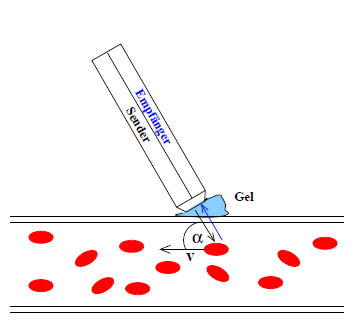
\includegraphics[width=0.5\linewidth]{Ultraschall.png}
	\caption{Die Anwendung des Dopplereffekts in der Ultraschalltechnik, \cite[1]{anleitungUS3}.}
	\label{fig:ultraschall}
\end{figure}
In der Abbildung \ref{fig:ultraschall} ist ein Beispiel dargestellt zur Anwendung des Dopplereffekts zur Bestimmung des Blutflusses in der Ultraschalltechnik. 
Tritt ein Ultraschall eine kommende Frequenz auf ein rotes bewegtes Blutkörperchen, so verschiebt sich die Frequenz wie beim Doppler-Effekt.
Die Formel lautet:
\begin{equation}
\label{eq:eq3}
\Delta \nu = \nu_0 \frac{v}{c}(\text{cos}\alpha + \text{cos}\beta),
\end{equation}
wobei $v$ die Geschwindigkeit des Objektes, $c$ die Schallgeschwindigkeit, die durch die Winkel $\alpha$ und $\beta$ bestimmt werden kann. 
Diese sind gleich beim Impuls-Echo-Verfahren, so dass es sich für die Formel \ref{eq:eq3} ergibt:
\begin{equation}
\label{eq:eq4}
\Delta \nu = 2 \nu_0 \frac{v}{c} \text{cos}\alpha
\end{equation}

Ultraschall kann durch technische Anordnungen erzeugt werden, zum Beispiel durch den piezoelektrischen-Effekt. Dieser kommt zustande, weil im elektrischen Feld einen Kristall gebracht wird, so dass dieser zu Schwingungen angeregt wird. 
Der Kristall kann auch als Detektor benutzt werden, dabei treffen die Schallwellen auf den Kristall und regen diesen zu Schwingungen an.